\documentclass[pub]{apa6}
\usepackage{apacite}
\usepackage{tipa}
\usepackage{graphicx}


\title{The Quenya Language}
\author{Anonymous}
\affiliation{Middle Earth}
\date{12 April 2013}
\shorttitle{Quenya}

\abstract{
Quenya is a fictional language devised by J. R. R. Tolkien, and used by the Elves in his fictional universe that is commonly known as Middle-earth. Tolkien began devising the language at around 1910 and re-structured the grammar several times until Quenya reached its final state. The vocabulary remained relatively stable throughout the creation process. Also the name of the language was repeatedly changed by Tolkien from Elfin and Qenya to the eventual Quenya. The Finnish language has been a major source of inspiration but Tolkien was also familiar with Latin, Greek and ancient Germanic languages when he began constructing Quenya. Another notable feature of Tolkien's Elvish languages was his development of a complex internal history of characters to speak those tongues in their own fictional universe since he felt that, as with the historical languages he studied professionally, his languages changed and developed over time not in a vacuum, but as a result of the migrations and interactions of the peoples who spoke them.
}

\begin{document}
\maketitle
\abstract


\section{Introduction}
J. R. R. Tolkien began to construct his first Elven tongue c. 1910-1911 while he was at the King Edward's School,
Birmingham. He later called it Qenya (c. 1915), and later changed the spelling to Quenya. He was then already
familiar with Latin, Greek, Spanish, and several ancient Germanic languages, such as Gothic, Old Norse and Old
English. He had invented several cryptographic codes, and two or three constructed languages. Taking an interest in the Finnish mythology of the Kalevala, Tolkien then became acquainted with the Finnish language, which he found to provide an aesthetically pleasing inspiration for his High-elven language.\\
\indent Many years later he wrote: ``It was like discovering a complete wine-cellar filled with bottles of an amazing wine of a kind and flavour never tasted before. It quite intoxicated me," \cite{tolkien2000}. Regarding the inspiration for Quenya he wrote that:
\begin{quotation}
The ingredients in Quenya are various... Finnish, which I came across when I had first begun to construct a 'mythology' was a dominant influence, but that has been much reduced [now in late Quenya]. It survives in some features: such as the absence of any consonant combinations initially, the absence of the voiced stops b, d, g (except in mb, nd, ng, ld, rd, which are favoured) and the fondness for the ending -inen, -ainen, -oinen, also in some points of grammar, such as the inflexional endings -sse (rest at or in), -nna (movement to, towards), and -llo (movement from); the personal possessives are also expressed by suffixes; there is no gender. \cite{tolkien1964}
\end{quotation}
Tolkien never intended Quenya, or any of his constructed languages, to be used in everyday life as an international auxiliary language, although he was in favour of the idea of Esperanto as an auxiliary language within Europe. With his Quenya, Tolkien pursued a double aesthetic goal: ``classical and inflected" \cite{tolkien1964}. \\
\indent This urge, in fact, was the motivation for his creation of a `mythology'. While the language developed, Tolkien felt that it needed speakers, including their own history and mythology, which he thought would give a language its `individual flavour' \cite{tolkien1968}. He wrote: "It was primarily linguistic in inspiration and was begun in order to provide the necessary background of `history' for Elvish tongues," \cite{tolkien1968}. This process of first inventing a language and then creating a background setting for its fictional speakers has been described as unique. \\
\indent Dimitra Fimi, a Tolkien scholar, argues that Tolkien's invention of Qenya started as a quest for the ideal language, to match the moral and aesthetic objectives that were part of his project of creating ``a mythology for England". Fimi argues that Tolkien deliberately used sound symbolism to unify sound and meaning and make the language appear as an ideal language, fit to be spoken in the utopian realm of the Elves and fairies of Valinor. Tolkien considered Quenya to be ``the one language which has been designed to give play to my own most normal phonetic taste.'' From the onset, Tolkien used comparative philology and the tree model as his major tools in his constructed languages. He usually started with the phonological system of the proto-language and then proceeded by inventing for each daughter language the necessary sequence of sound changes. In a letter to a reader, he writes: "I find the construction and the interrelation of Quenya and the languages an aesthetic pleasure in itself, quite apart from The Lord of the Rings, of which it was/is in fact independent," \cite{tolkien1964b}.

\section{Development}
In his lifetime, J. R. R. Tolkien never ceased to experiment on his constructed languages, and they were subjected to many revisions. Therefore Quenya had many grammars with substantial differences between the different stages of its development. During the first conceptual stage of early Quenya c. 1910 to c. 1920, the language was called {\it Elfin} in English and {\it Eldarissa} in Qenya proper. While its development was a continuous process, Quenya underwent a number of major revisions in its grammar, mostly in conjugation and the pronominal system. The vocabulary, however, was not subject to sudden or extreme change. Tolkien sometimes changed the meaning of a word, but he almost never discarded it once invented, and he kept on refining its meaning, and countlessly forged new synonyms. Moreover, Elvish etymology was in constant flux. Tolkien delighted in inventing new etonyms for his Quenya vocabulary. But after the publication of The Lord of the Rings (1954-1955), the grammar rules of Quenya went through very few changes and this version was then defined as late Quenya (1954-1973).\\
\indent The spelling Qenya is sometimes used to distinguish early Quenya from later versions. Qenya differs from late Quenya by having different internal history, vocabulary, and grammar rules as described in the ``Qenyaqetsa". Examples include a different accusative or the abolition of final consonant clusters in later Quenya. Fimi suggests that Qenya as it appears in the ``Qenyaqetsa" was supposed to be a mystic language, as the Lexicon contains a number of words with clear Christian religious connotations, such as anatarwesta ``crucifixion" and evandilyon ``gospel" \textendash\  these words were not part of late Quenya.\\
\indent In the early 1930s, Tolkien decided that the proto-language of the Elves was Valarin, the tongue of the gods or Valar as he called them: ``The language of the Elves derived in the beginning from the Valar, but they changed it even in the learning, and moreover modified and enriched it constantly at all times by their own invention." In the Comparative Tables the mechanisms of sound change were described by Tolkien for the following daughter languages: {\it Qenya}, {\it Lindarin} (a dialect of Qenya), {\it Telerin}, {\it Old Noldorin} (or Fëanorian), {\it Noldorin} (or Gondolinian), {\it Ilkorin} (especially of Doriath), {\it Danian} of Ossiriand, {\it East Danian}, {\it Taliska}, {\it West Lemberin}, {\it North Lemberin}, and {\it East Lemberin}. For this proto-language of the Elves, Tolkien appears to have borrowed the five-part plosive system of Proto-Indo-European, the ancestor of Latin, Greek, Sanskrit, and others; namely, one labial, one coronal, and three velar plosives (palatal, plain, and labial). The first table below provides some of the ``Primary Initial Combinations" from the Comparative Tables.\\

\begin{figure}
\bigskip
\begin{tabular}{|l|l|l|l|} \hline	
{\bf Valarin}	&	{\bf Qenya}				&	{\bf Lindarin}	&	{\bf Telerin}		\\ \hline
mb				&	m, umb 					&	m, umb			&	m, emb				\\ \hline
nd				&	n, and					&	n, and			&	n, end				\\ \hline
\textipa{N}gj 	& 	ny, indy, iny			&	\~n, ind		& 	g, ang				\\ \hline
\textipa{N}g 	&	\textipa{N} > n, ing	&	n, ing			&	\textipa{N}g, eng	\\ \hline
\textipa{N}gw 	& 	\textipa{N}w > nw, ungw & 	m, ungw 		&	m, emb				\\ \hline		
\end{tabular}
\bigskip
\caption{Comparative table of initial nasal consonants in Elven languages}
\end{figure}
Another characteristic of Quenya reminiscent of ancient natural languages like Old Greek, Old English or Sanskrit is the dual grammatical number which is used in addition to singular and plural. It has been suggested that Tolkien used the dual to give Quenya an ``archaic feel'' in its role as an ancient language of the Elves.\\
\indent About ten years later, Tolkien changed his mind about the origin of the Elvish proto-language. Instead of learning from the Valar, the Elves had created an original language {\it Quenderin} which had become the proto-language of the Elven language family. For this new language, Tolkien kept the many roots he had invented for Valarin in the 1930s, which then became ``Quenderin roots''. The Eldarin family of languages comprises Quenya, Telerin, Sindarin and Nandorin. The evolution in Quenya and Telerin of the nasalized initial groups of Quenderin is described thus in Tolkien's {\it Outline of Phonology}.\\
\indent In contrast to early Qenya, the grammar of Quenya was influenced by Finnish, an agglutinative language, but much more by Latin, a synthetic and fusional language, and also Greek, from which he probably took the idea of the diglossia of Quenya with its highly codified variety: the {\it Parmaquesta}, used only in certain situations such as literature. Also the phonology of Quenya was inspired by certain aspects of Finnish, but this is not easily
recognized.\\
\indent Tolkien almost never borrowed words directly from real languages into Quenya. The major exception is the name {\it Earendel/E\"arendil}, which he found in an Old English poem by Cynewulf. Yet the Finnish influence extended sometimes also to the vocabulary. A few Quenya words, such as {\it tul-} `come' and {\it anta-} `give', clearly have a Finnish origin. Other forms that appear to have been borrowed are actually coincidental, such as Finnish {\it kirja} `book', and Quenya {\it cirya} `ship'. Tolkien invented the Valarin/Quenderin root {\it kir-} from which sprang his Quenya word cirya. The Latin {\it aure} `dawn', and Quenya {\it aure} ``moment of special meaning, special day, festival day'' are unrelated. Instead, Quenya {\it aure} comes from the Valarin/Quenderin root {\it ur-}. Germanic influence can more be seen in grammar
(the {\it -r} nominative plural ending is reminiscent of the Scandinavian languages) or phonology, than in words: {\it Arda}, the Quenya name for `region', just happened to resemble Germanic {\it Erde} `earth', while it actually comes from the Valarin/Quenderin root {\it gar-}. According to Tom DuBois and Scott Mellor, the name of Quenya itself may have been influenced by the name Kven, a language closely related to Finnish, but Tolkien never mentioned this.\\
\indent Some linguists have argued that Quenya can be understood as an example of a particular kind of artificial language that helps to create a fictional world. Other such languages would include Robert Jordan's Old Tongue and the Klingon language of the Star Trek series invented by Marc Okrand. It was observed that they form ``a sociolinguistic context within which group and individual identities can be created.''

\subsection{Publication of linguistic papers}
Two journals, {\it Vinyar Tengwar} from issue No. 39 (July 1998), and {\it Parma Eldalamberon} from issue No. 11 (1995), are today exclusively devoted to the editing and publishing of J. R. R. Tolkien's mass of unpublished linguistic papers. Important grammatical texts, alluded to by Christopher Tolkien in his {\it History of Middle-earth} series and described as almost unreadable or quite incomprehensible, have been published in these two journals. The ``Early Qenya Grammar'', written by J. R. R. Tolkien c. 1925, was successfully edited and published in {\it Parma Eldalamberon} No. 14.\\
\indent The editors have not published a comprehensive catalogue of the linguistic papers they are working on and that were not published by Christopher Tolkien in the {\it History of Middle-earth}; new Tolkienian linguistic material continues to emerge, although the pace of publication is irregular.

\subsection{Use of Quenya}
Attempts by fans to write in Quenya began in the 1970s, when the total corpus of published Elvish comprised only a few hundred words. Since then, the use of Elvish has flourished in poems and texts, phrases and names, and even tattoos. But Tolkien himself never made his languages complete enough for conversation. As a result, newly invented Elvish texts require conjecture and sometimes the coinage of new words. The use of Quenya has
expanded over the years as new words have been created, forming a {\it Neo-Quenya} language that is based on Tolkien's original Quenya but incorporates many new elements.

\section{Internal History}
The Elvish languages are a language family of several related languages and dialects. The following is a brief
overview of the fictional internal history of Quenya as conceived by Tolkien c. 1965. Tolkien imagined a diglossic Elven society with a vernacular language for every-day use, {\it Tarquesta}, and a more educated language for use in ceremonies and lore, {\it Parmaquesta}.\\
\indent It has been observed that the ``degree of proximity'' to the light of the Valar affects the development of both languages in terms of phonology, morphology and semantics. The division between Light Elves and Dark Elves that took place during the Sundering of the Elves is reflected in their respective languages.\\
\indent The Elves at first shared a common language, Primitive Quendian, called Quenderin in Quenya. Among the Eldar, i.e. those Elves who undertook the Great March to Valinor and Eldamar, Primitive Quendian developed into Common Eldarin. Some of the Eldar remained in Beleriand and became the Grey Elves; their language developed into Sindarin. Most of the other Eldar continued to Eldamar ('Elvenhome') and founded the great city of Tirion, where they developed Quenya.\\
\indent Quenya's older form, first recorded in the sarati of R\'umil, is called Old or Ancient Quenya (Y\'ara-Quenya in Quenya). In Eldamar, the Noldor and Vanyar spoke two slightly different though mutually intelligible dialects of Tarquesta: Noldorin Quenya and Vanyarin Quenya. Later Noldorin Quenya became Exilic Quenya, when most of the Noldor Elves followed their leader F\"eanor into exile from Eldamar and back to Middle-earth, where the immortal Elves first awoke.\\
\indent Quenya was also used by the gods or Valar. The Elves even derived some loanwords from the Valar's language, which was called Valarin in Quenya, although these were more numerous in the Vanyarin dialect than in Noldorin. This was probably because of the enduringly close relationship the Vanyarin Elves had with the Valar. The Quenya as used by the Vanyar also incorporated several words from Valarin that were not found in the Noldorin dialect, such as {\it tulka} (`yellow', from Valarin {\it tulukha(n)}), {\it ulban} (`blue', presumably from the same root as Valarin {\it ul(l)u} meaning `water'), and {\it nasar} (`red', original Valarin not given).\\
\indent According to ``Quendi and Eldar: Essekenta Eldarinwa'', written by \AE lfwine, Quendya was the usual Vanyarin name given to the Quenya language, since in Vanyarin, the consonant groups /ndy/ and /ny/ remained quite distinct. In Noldorin, /ndy/ eventually became /ny/. Tolkien explained that ``the word Quenya itself has been cited as an exempla (e.g. by \AE lfwine), but this is a mistake due to supposition that {\it kwenya} was properly {\it kwendya} and directly derived from the name Quendi `Elves'. This appears not to be the case. The word is Quenya in Vanyarin, and always so in Parmaquesta.''\\
\indent The Elves of the Third Clan, or {\it Teleri}, who reached Eldamar later than the Noldor and the Vanyar, spoke a different but closely related tongue, usually called Telerin. It was seen by some Elves to be just another dialect of Quenya. This was not the case with the Teleri for whom their tongue was distinct from Quenya. After the Vanyar left the city of T\'una, Telerin and Noldorin Quenya grew closer.\\
\indent The rebellious Noldor, who followed their leader F\"eanor to Middle-earth, spoke only Quenya. But Elu Thingol, King of the Sindar of Beleriand, forbade the use of Quenya in his realm when he learned of the slaying of Telerin Elves by the Noldor ({\it The Silmarillion}, chapter 15). By doing so, he both restricted the possibility of the Sindar to enhance and brighten their language with influences from Quenya and accelerated the ``dimininuation and spiritual impoverishment'' of the Noldorin culture. The Noldor at this time had fully mastered Sindarin, while the Sindar were slow to learn Quenya. Quenya in Middle-earth became known as Exilic Quenya when the Noldor eventually adopted the Sindarin language as their native speech after Thingol's ruling. It differed from Amanian Quenya mostly in vocabulary, having some loanwords from Sindarin. It differed also in pronunciation, representing the recognition of sound-changes which had begun among the Noldor before the exile and had caused Noldorin Quenya to diverge from Vanyarin Quenya. The change of {\it z} (< old intervocalic {\it s}) to {\it r} was the latest in Noldorin, belonging to early Exilic Quenya. The grammatical changes were only small though since the features of their ``old language'' were carefully taught.\\
\indent From the Second Age on, Quenya was also used ceremonially by the Men of N\'umen\'or and their descendants in Gondor and Arnor for the official names of kings and queens; this practice was resumed by Aragorn when he took the crown as Elessar Telcontar. Quenya in the Third Age had almost the same status as the Latin language had in medieval Europe, and was called Elven-latin by Tolkien.

\section{Writing Systems}
\indent Most of the times, Tolkien wrote his invented languages using the Latin script, but he devised a number of original writing systems to match the internal histories of his languages.\\

\subsection{Elvish writing system}
Tolkien imagined many writing systems for his Elves. The most well-known is the ``Tengwar of F\"eanor'' but the first one he created c. 1919 was the ``Tengwar of Rumil'', also called the {\it sarati}. He decided that, prior to their Exile, the Noldorin Elves first used the sarati of R\'umil to record Ancient Quenya. In Middle-earth, Quenya appears to have been rarely written using the ``Elvish runes'' or {\it cirth}, named {\it certar} in Quenya.\\

\subsection{Latin alphabet}
Tolkien's spelling in Latin letters of Quenya was largely phonemic, with each letter corresponding to a specific phoneme in the language, save for some exceptions. In particular, the vowels varied in pronunciation depending upon their vowel length. Specific rules for consonants were provided in Appendix E of {\it The Lord of the Rings}, e.g. the letter {\it c} is always pronounced [k], {\it qu} stands for [kw], Orqui is Orkwi. Occasionally, Tolkien wrote Quenya with a "Finnish-style" orthography (rather than the standard Latin-Romance version), in which {\it c} is replaced by {\it k}, {\it y} with {\it j}, and long vowels written double.\\

\begin{figure}
\bigskip
\begin{center}
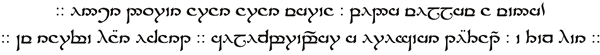
\includegraphics[width=80mm, height=10mm]{sindarin.png}
\end{center}
\caption{Sindarin script on Gate of Moria, reads: ``Gate of Durin, King of Moria, say friend and enter!  I, Narvi made them. Celebrimbor of Eregion drew these signs.''}
\end{figure}

\section{Corpus}
The poem ``Nam\'ari\"e'' is the longest piece of Quenya found in {\it The Lord of the Rings}, yet the first sentence in Quenya is uttered by a Hobbit; namely Frodo's greeting to the Elves: {\it elen s\'ila l\'umenn omentielvo}. Other examples include Elendil's words spoken upon reaching Middle-earth, and repeated by Aragorn at his coronation: {\it Et E\"arello Endorenna ut\'ulien. Sinom\"e maruvan ar Hildinyar tenn Ambar-metta!} ``Out of the Great Sea to Middle-earth I am come. In this place I will abide, and my heirs, unto the ending of the world!'' Treebeard's greeting to Celeborn and Galadriel is also spoken in Quenya: {\it A vanimar, vanim\'alion nostari} ``O beautiful ones, parents of beautiful children.'' Another fragment is Frodo's cry when he uses Galadriel's phial against Shelob: Aiya E\"arendil Elenion Ancalima! ``Hail E\"arendil, brightest of stars!'' And in {\it The Silmarillion}, the phrase {\it Ut\'ulie'n aur\"e! Aiya Eldali\"e ar Atanat\'ari, ut\'ulie'n aur\"e!} ``The day has come! Behold, people of the Eldar and Fathers of Men, the day has come!'', is cried by Fingon before the Battle of Unnumbered Tears.

\bibliographystyle{apacite}
\bibliography{quenya}

\end{document}